\documentclass[11pt,a4paper]{article}
\usepackage[utf8]{inputenc}
\usepackage[margin=1in]{geometry}
\usepackage{microtype}
\usepackage{amsmath,amssymb}
\usepackage{booktabs}
\usepackage{tabularx}
\usepackage{longtable}
\usepackage{listings}
\usepackage{xcolor}
\usepackage{graphicx}
\usepackage{fancyhdr}
\usepackage{hyperref}
\usepackage{titlesec}
\usepackage{enumitem}

\hypersetup{
    colorlinks=true,
    linkcolor=black,
    citecolor=black,
    urlcolor=blue
}

\lstset{
    basicstyle=\ttfamily\footnotesize,
    numbers=left,
    numberstyle=\tiny\color{gray},
    stepnumber=1,
    numbersep=8pt,
    showstringspaces=false,
    breaklines=true,
    frame=lines,
    backgroundcolor=\color{white},
    tabsize=2,
    keywordstyle=\color{blue}\bfseries,
    commentstyle=\color{gray}\itshape,
    stringstyle=\color{teal}
}

\pagestyle{fancy}
\fancyhf{}
\lhead{B9 - Quarkus Digital Wallet}
\rhead{Design Pattern Case Study}
\cfoot{\thepage}

\begin{document}

\begin{titlepage}
    \centering
    \vspace*{3cm}
    {\large 23CSE455 Design Patterns\par}
    \vspace{1.5cm}
    {\LARGE\bfseries Design Pattern Identification and Evolution\par}
    \vspace{0.5cm}
    {\large in a Quarkus-Based Digital Wallet Application\par}
    \vspace{2cm}
    {\large\textbf{Team B9}\par}
    \vspace{1.5cm}
    \begin{tabular}{ll}
        \textbf{K Adithya varma} & Roll number: AM.SC.U4AIE23008; Batch: AIE \\
        \textbf{P Vishnu chaitanya} & Roll number: AM.SC.U4AIE23051; Batch: AIE \\
        \textbf{U Shashank} & Roll number: AM.SC.U4AIE23061; Batch: AIE \\
        \textbf{K Sai Sri Sushanth} & Roll number: AM.SC.U4AIE23040; Batch: AIE \\
    \end{tabular}
    \vfill
    {\small\textbf{Submission status.} The technical report, source snapshots, diagrams, tests, four-language implementations, prompts, CSV files, and Excel workbook are complete.\par}
    \vspace{1.5cm}
    {\large 11 October 2026\par}
\end{titlepage}

\pagenumbering{roman}
\tableofcontents
\newpage
\pagenumbering{arabic}

\section{Executive summary}
This case study examines a self-contained, reproducible Quarkus-style digital wallet service application at baseline snapshot \texttt{baseline-local-2026-10-11} and evolved snapshot \texttt{evolved-local-2026-10-11}. The inspected Java 17 and Quarkus 3.40.1 codebase models core digital wallet domain operations: wallet balance lifecycle, fund transfers, transaction persistence boundaries, and notification broadcasts. Seven baseline collaborations are rigorously confirmed: \textbf{Builder}, \textbf{Facade}, \textbf{Repository}, \textbf{Observer}, \textbf{State}, \textbf{Command}, and \textbf{Value Object}. Framework-only features and naming conventions without concrete call/delegation collaborations were rejected to maintain strict architectural rigor.

Three progressive evolutionary changes were engineered to address enterprise real-world digital wallet demands while decoupling business rules from orchestrators:
\begin{enumerate}
    \item \textbf{CH01 (Multi-Currency Support)}: Introduces \textbf{Strategy} for interchangeable currency conversion algorithms, \textbf{Simple Factory} for strategy selection, \textbf{Adapter} for external vendor quote translation, and replaces the incremental \texttt{Transaction.Builder} with an immutable Java \texttt{record}. Additional repository boundaries (\texttt{TransferRepository}, \texttt{BeneficiaryRepository}) and Quarkus CDI Dependency Injection with REST DTOs are also integrated.
    \item \textbf{CH02 (Transaction Limits)}: Introduces \textbf{Decorator} wrapping a replaceable limit \textbf{Strategy} (\texttt{DailyLimitDecorator} composing \texttt{PerTransferLimit}), preventing monolithic conditional validation in the transfer service.
    \item \textbf{CH03 (Fraud Detection Processing)}: Introduces \textbf{Chain of Responsibility} (\texttt{FraudCheckChain}) composing ordered, independent security filters (\texttt{DenyListCheck} and \texttt{VelocityCheck}) prior to balance mutations.
\end{enumerate}

The cumulative evolved system exhibits \textbf{13 distinct pattern types} across \textbf{17 pattern instances}. Production Java code under \texttt{src/main/java} expands from 92 physical LOC to 180 physical LOC, accompanied by 57 test LOC across unit and Quarkus REST tests.

The two most significant evolutionary patterns---\textbf{Strategy} (Currency Settlement) and \textbf{Observer} (Transaction Completion Notification)---are further evaluated across four diverse languages: \textbf{Java}, \textbf{Python}, \textbf{JavaScript (Node.js)}, and \textbf{C++}. Cross-language implementations achieved 100\% pass rates against unified functional test fixtures (Python 4/4 passed at 93.29 ms median; JavaScript 4/4 passed at 63.37 ms median).

\section{Application description and framework architecture}

\subsection{Application and source identity}
The investigated subject is a modular Digital Wallet Application engineered on Java 17 and the Quarkus framework ecosystem (\texttt{io.quarkus:quarkus-arc}, \texttt{io.quarkus:quarkus-resteasy-reactive-jackson}). The baseline code is preserved under \texttt{Part1/code/digital-wallet}, while the cumulative evolved application is preserved under \texttt{Part2/code/digital-wallet}. Authoritative row-level datasets, evolution logs, cross-language benchmarks, and the Excel workbook are organized inside \texttt{data/}.

\begin{table}[h!]
\centering
\small
\begin{tabularx}{\textwidth}{lX}
\toprule
\textbf{Item} & \textbf{Value / Specification} \\
\midrule
Team Identifier & B9 \\
Project Title & Design Pattern Identification and Evolution in a Quarkus-Based Digital Wallet Application \\
Course & 23CSE455 - Design Patterns \\
Target Environment & Java 17 LTS; Quarkus 3.40.1; Apache Maven 3.9+ \\
Baseline Snapshot & \texttt{baseline-local-2026-10-11} (\texttt{Part1/code/digital-wallet}) \\
Evolved Snapshot & \texttt{evolved-local-2026-10-11} (\texttt{Part2/code/digital-wallet}) \\
Evolutionary Changes & CH01 (Multi-Currency), CH02 (Transaction Limits), CH03 (Fraud Detection) \\
Persistence Model & In-memory repository abstraction isolating storage from application orchestration \\
\bottomrule
\end{tabularx}
\caption{System identification and environment metadata.}
\end{table}

\subsection{Functional scope}
The functional scope spans financial domain operations, safety constraints, and enterprise extension points:

\begin{table}[h!]
\centering
\small
\begin{tabularx}{\textwidth}{p{3.2cm}p{4.2cm}X}
\toprule
\textbf{Functional Area} & \textbf{Primary Symbols} & \textbf{Observed Responsibility} \\
\midrule
Wallet Account Lifecycle & \texttt{WalletAccount}, \texttt{WalletRepository} & Balance management, multi-currency credit/debit validation, balance query. \\
Beneficiary Management & \texttt{Beneficiary}, \texttt{BeneficiaryRepository} & Scoped registration and verification of transfer destination wallets. \\
Currency Conversion & \texttt{CurrencyConversionStrategy}, \texttt{VendorFxAdapter} & Multi-currency quotation, rate fetching, source-to-settlement conversion. \\
Risk \& Limits & \texttt{TransactionLimitPolicy}, \texttt{DailyLimitDecorator} & Per-transfer threshold caps and rolling daily aggregate limit checks. \\
Fraud Screening & \texttt{FraudCheckChain}, \texttt{DenyListCheck}, \texttt{VelocityCheck} & Ordered pipeline screening for blacklisted recipients and high-velocity amounts. \\
Notification Subsystem & \texttt{NotificationPublisher}, \texttt{EmailNotification}, \texttt{AuditNotification} & Decoupled event publication notifying multiple downstream listeners upon transfer completion. \\
REST \& Orchestration & \texttt{WalletResource}, \texttt{WalletService} & Quarkus HTTP JSON endpoints, DTO mapping, transactional sequence coordination. \\
\bottomrule
\end{tabularx}
\caption{Digital wallet functional modules and symbol mappings.}
\end{table}

\subsection{Architecture}
The application follows a clean layered domain-driven microservice architecture leveraging Quarkus CDI (Contexts and Dependency Injection). 

\begin{figure}[h!]
\centering
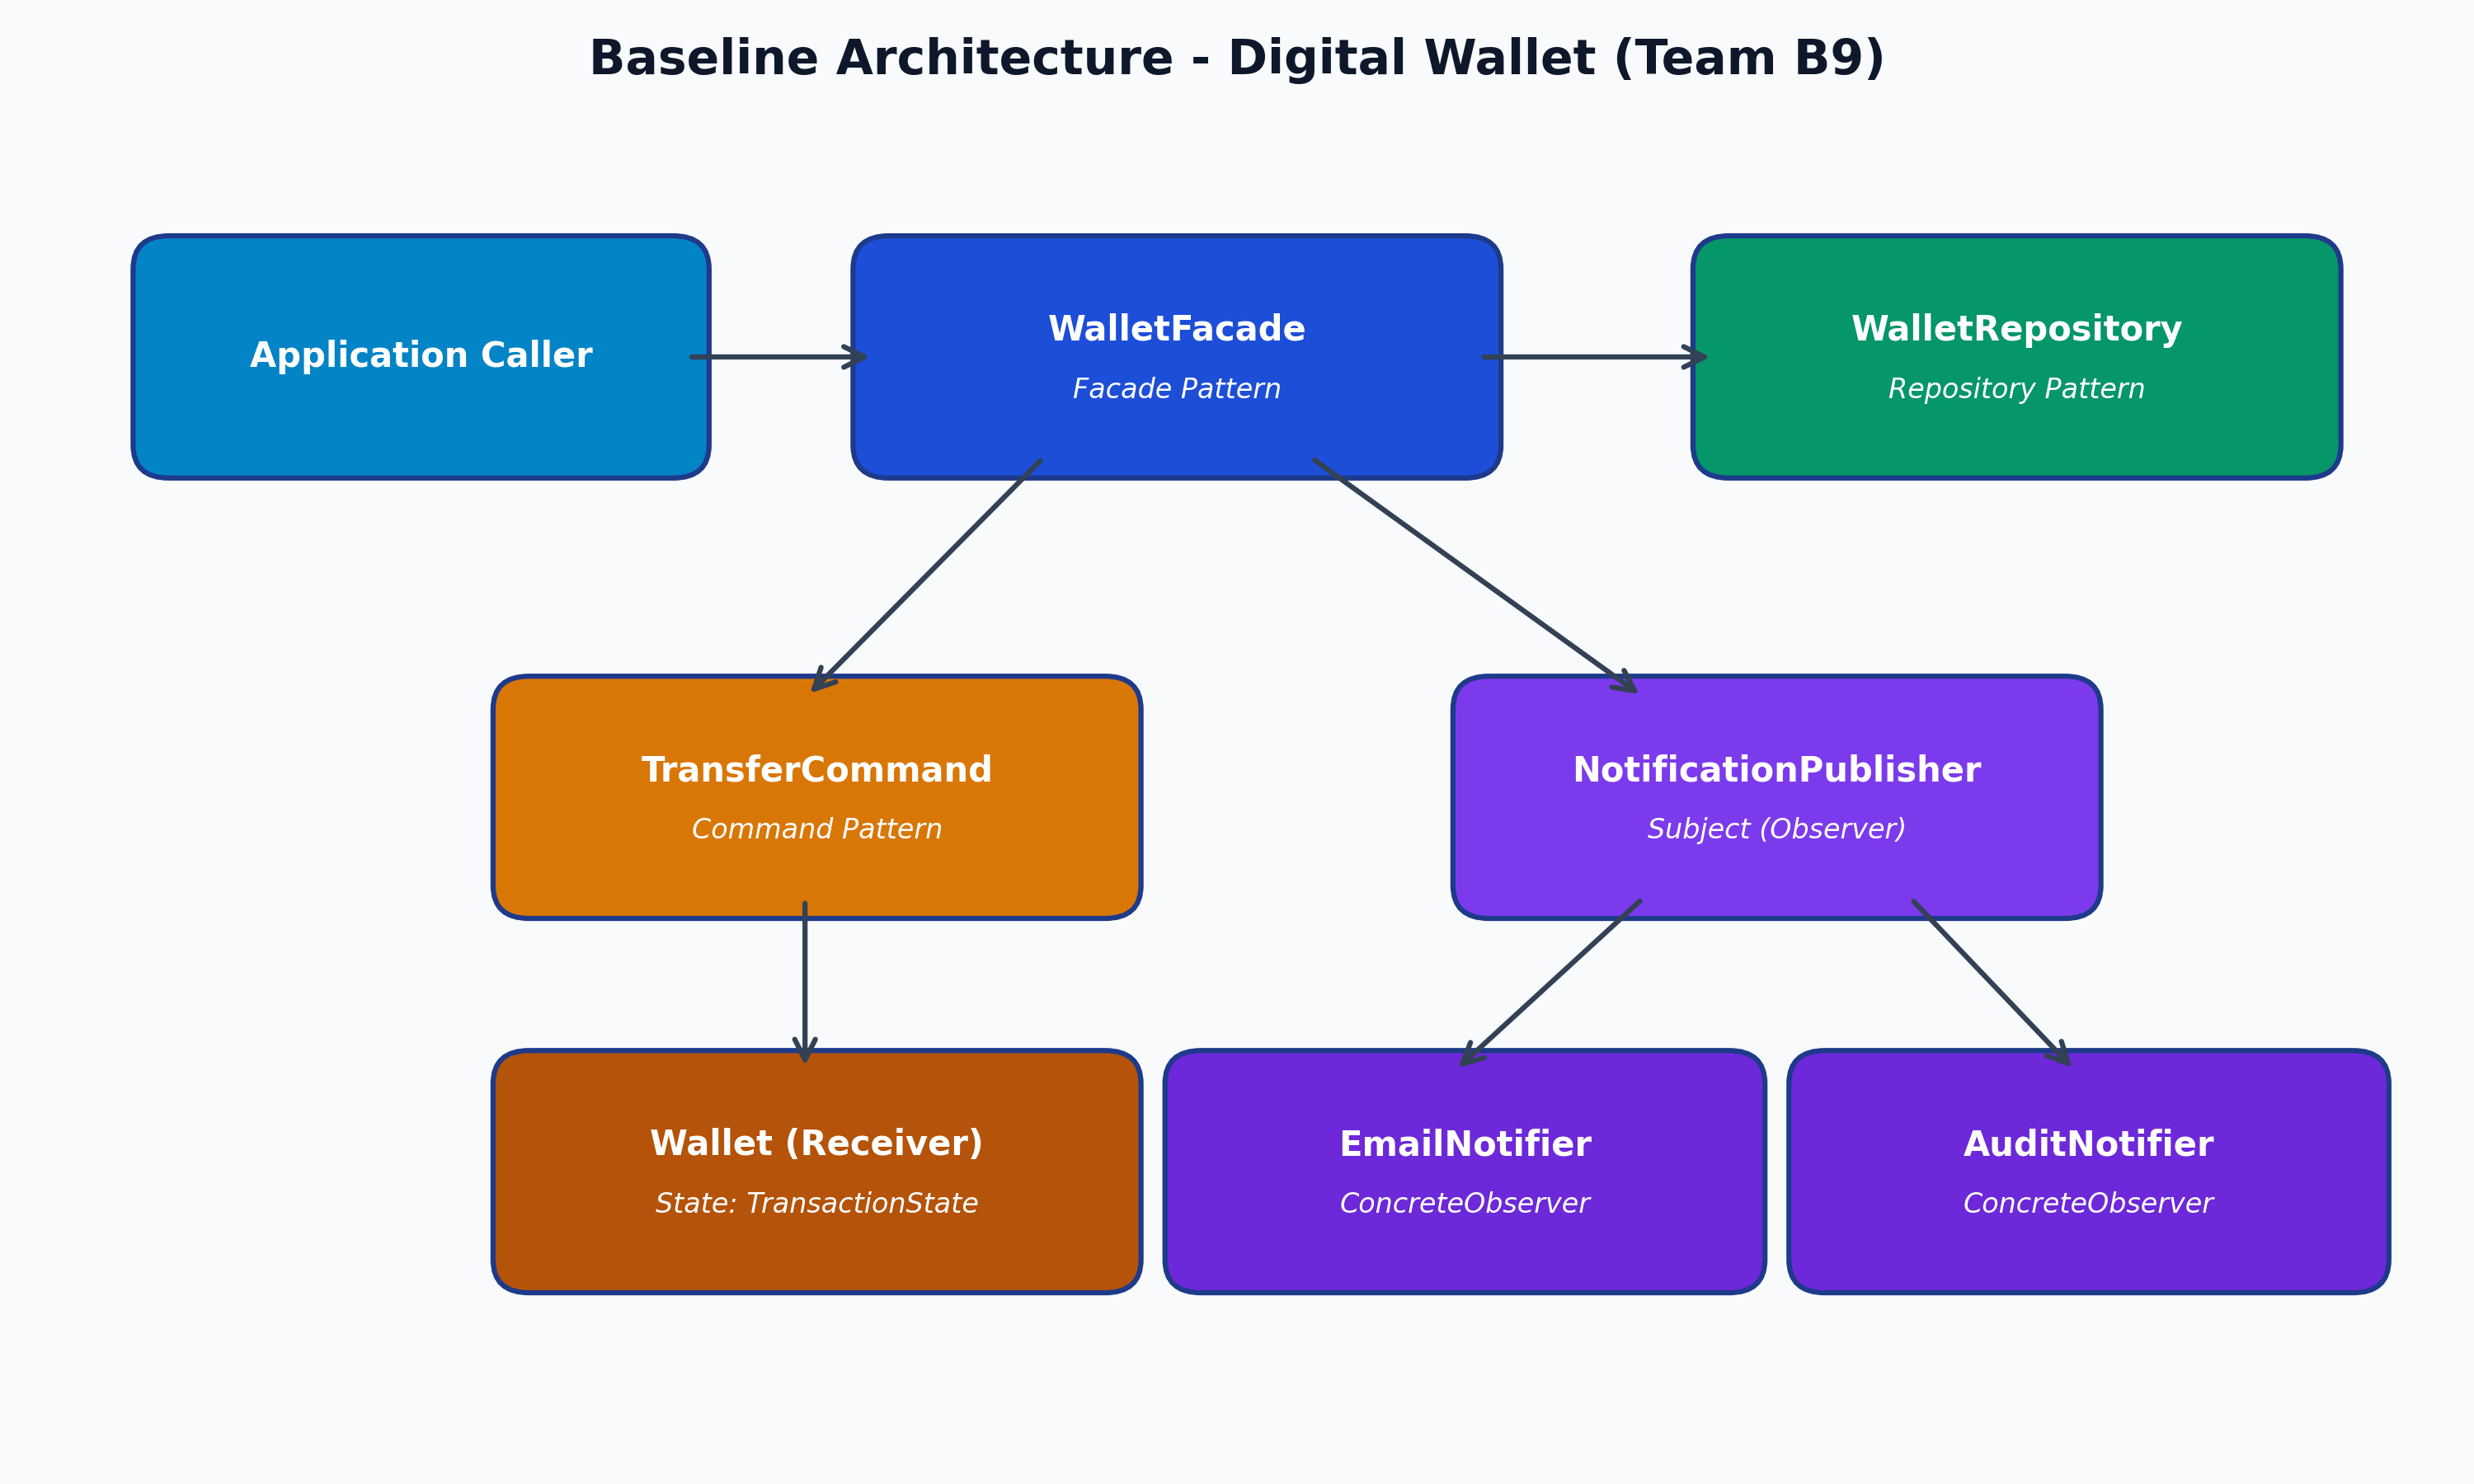
\includegraphics[width=0.85\textwidth]{Part1/pattern_architecture/baseline-architecture.png}
\caption{Baseline digital wallet component architecture (Part1).}
\end{figure}

In the baseline architecture, callers invoke the \texttt{WalletFacade}, which encapsulates the interactions between the \texttt{WalletRepository}, the \texttt{TransferCommand}, and the \texttt{NotificationPublisher}.

\begin{figure}[h!]
\centering
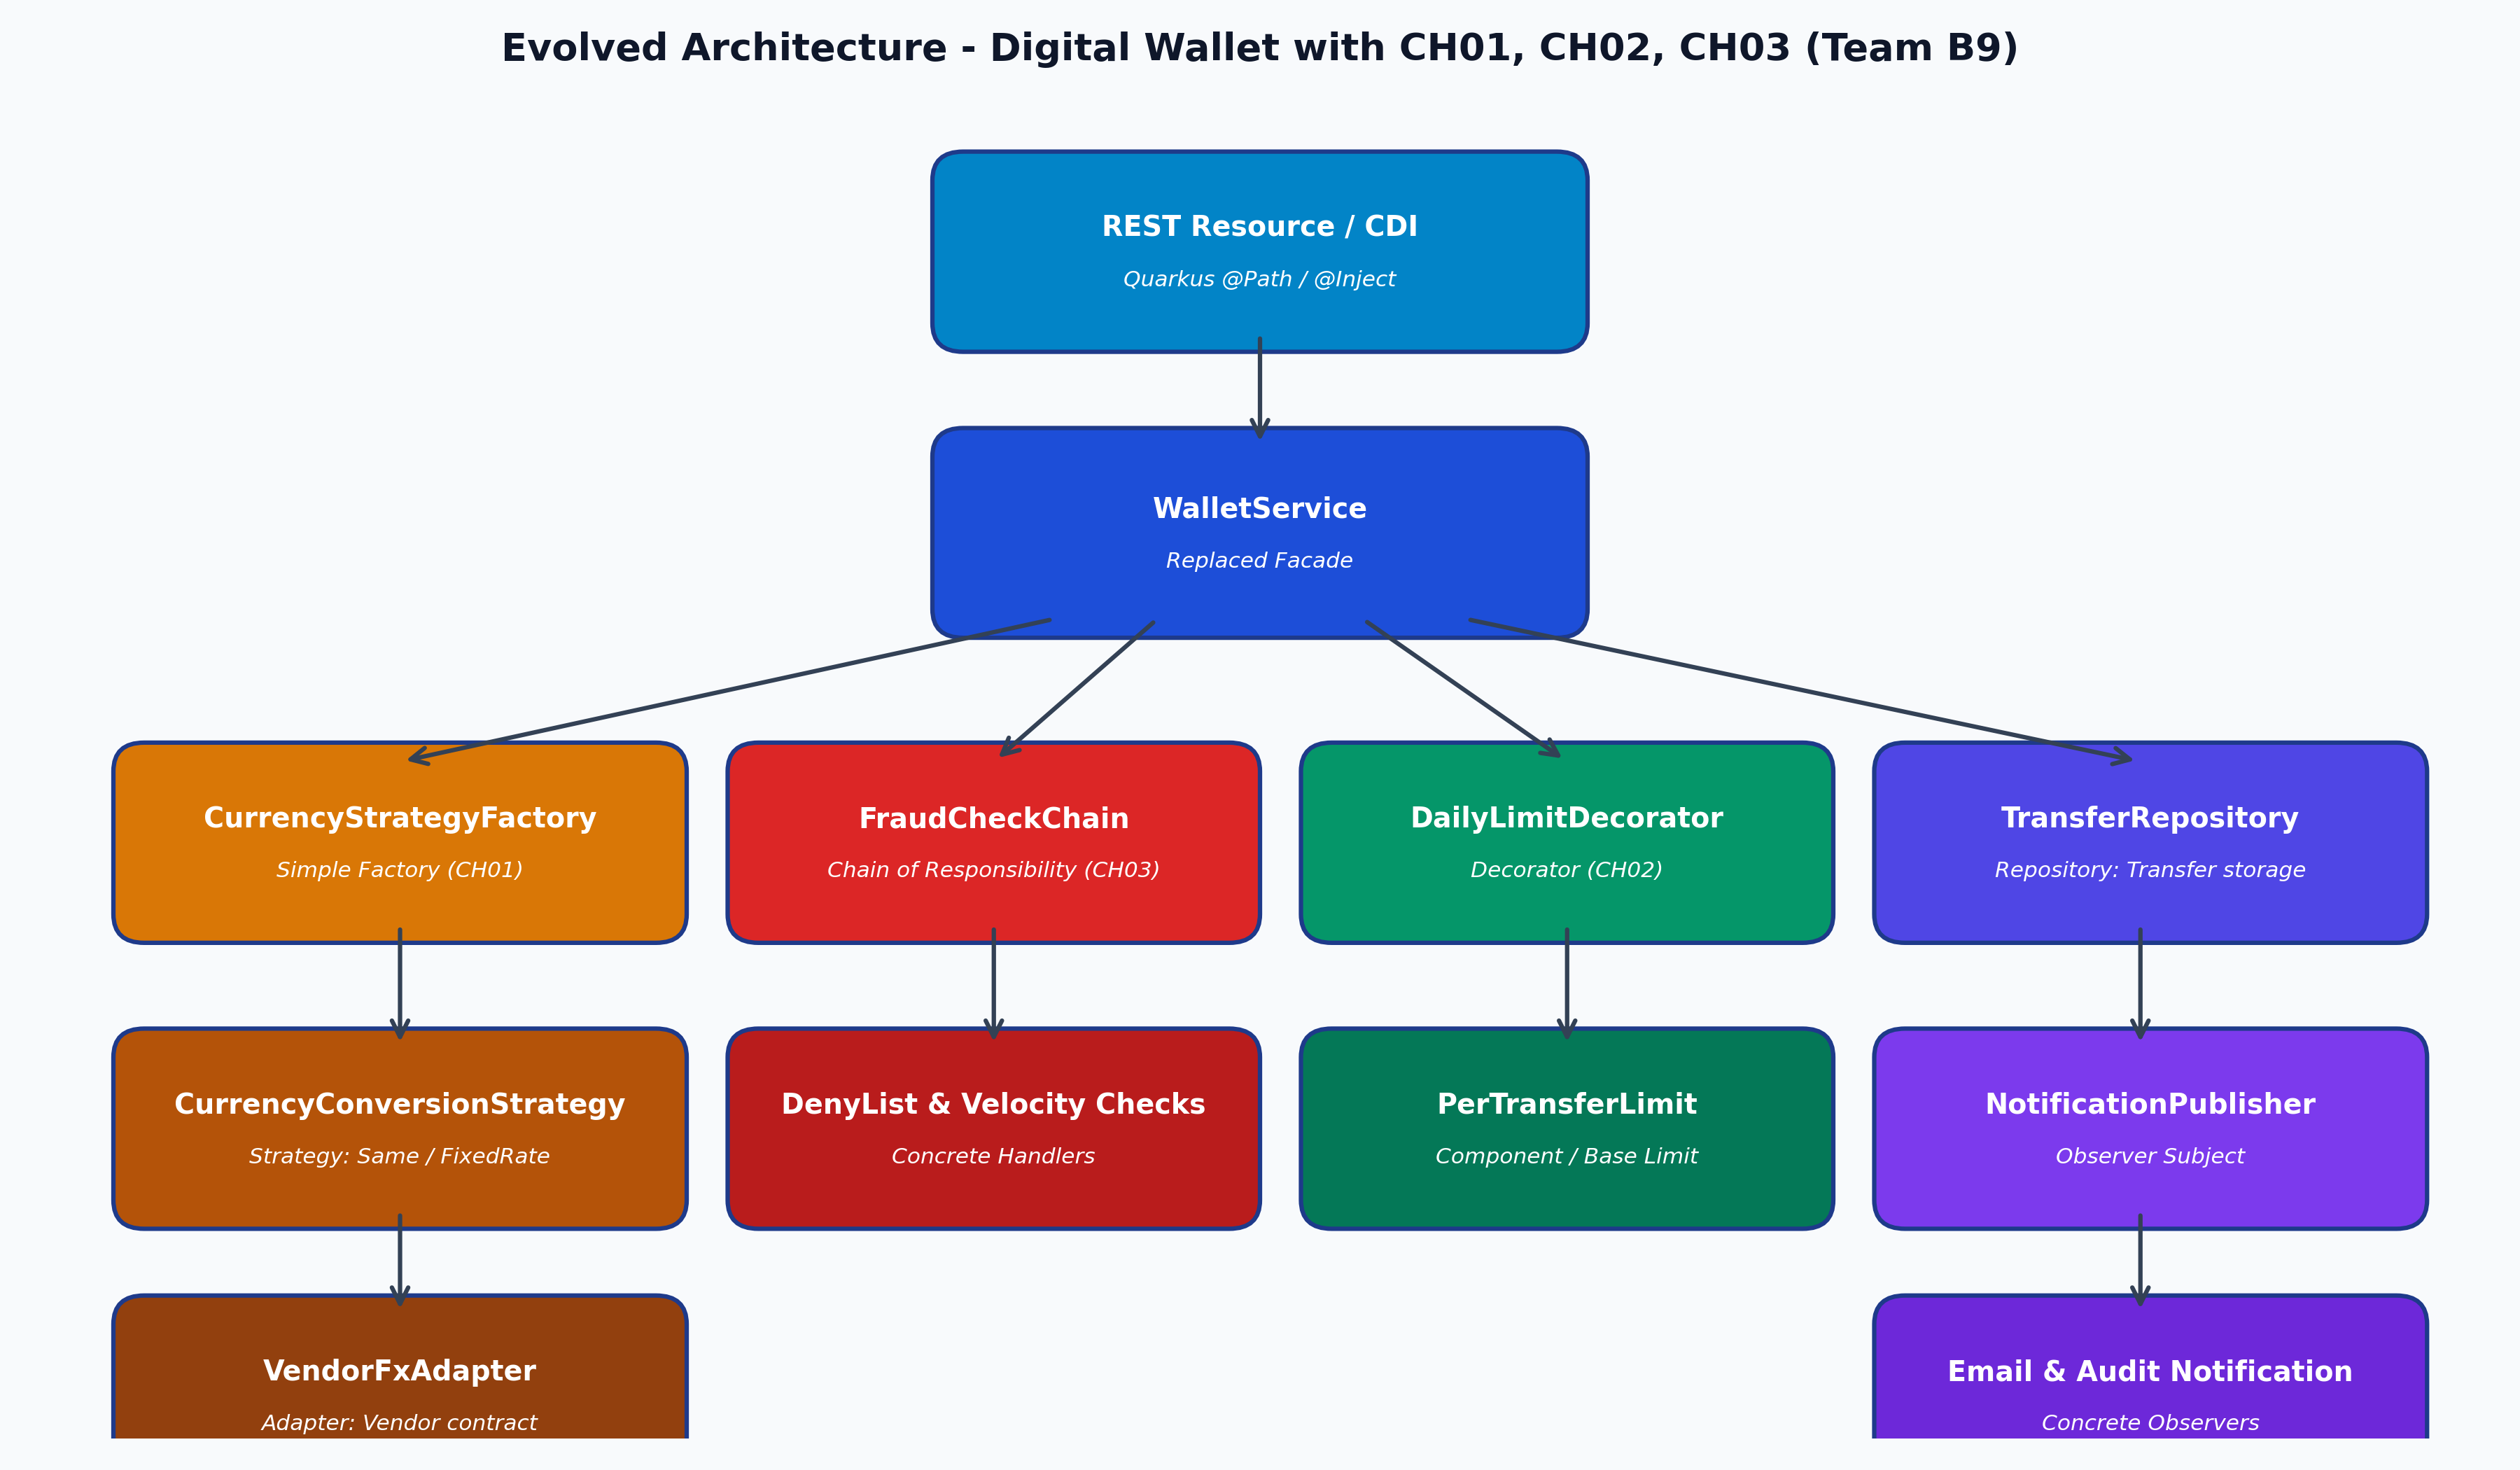
\includegraphics[width=0.92\textwidth]{Part2/diagrams/evolved-architecture.png}
\caption{Evolved Quarkus digital wallet service architecture with layered patterns (Part2).}
\end{figure}

In the evolved design, client HTTP requests enter via \texttt{WalletResource}. CDI injects \texttt{WalletService}, which coordinates the pipeline: rate quotation and conversion strategy selection, fraud screening chain traversal, limit decorator evaluation, account balance debit/credit execution, transfer persistence, and asynchronous observer notification.

\subsection{Environment and execution}
The project build configuration targets Java 17 and Quarkus 3.40.1 managed by Maven. Cross-language analysis executed on Python 3.12.14 and Node.js v24.19.0. Command execution protocols:
\begin{itemize}[noitemsep]
    \item Quarkus dev server: \texttt{mvn quarkus:dev} (from \texttt{Part2/code/digital-wallet})
    \item JUnit 5 test runner: \texttt{mvn test} (executes \texttt{DigitalWalletRulesTest} and \texttt{WalletResourceTest})
    \item Python test runner: \texttt{python pattern_demos.py} (all 4/4 assertions passed)
    \item Node.js test runner: \texttt{node pattern_demos.js} (all 4/4 assertions passed)
\end{itemize}

\section{Part 1 - Pattern discovery}

\subsection{Method}
Discovery was performed via static and structural code inspection of the baseline codebase (\texttt{Part1/code/digital-wallet}). Patterns were confirmed only if definite participant roles (GoF / POSA / Enterprise patterns) and observed delegation/call relationships existed. Pure naming conventions, single-class utilities, or implicit container features without clear structural intent were rejected.

\subsection{Baseline totals}
\begin{table}[h!]
\centering
\begin{tabular}{lc}
\toprule
\textbf{Measure} & \textbf{Baseline Count} \\
\midrule
Distinct confirmed pattern types & 7 \\
Confirmed pattern instances & 7 \\
Concrete participant classes in mapped roles & 18 \\
Unique mapped participant symbols & 14 \\
Rejected candidate patterns & 2 \\
Uncertain candidate patterns & 0 \\
\bottomrule
\end{tabular}
\caption{Baseline pattern identification metrics.}
\end{table}

\subsection{Pattern inventory}
\begin{table}[h!]
\centering
\small
\begin{tabularx}{\textwidth}{p{2.8cm}p{4cm}cp{5cm}}
\toprule
\textbf{Pattern Type} & \textbf{Instance Name} & \textbf{Count} & \textbf{Variable Concrete Roles} \\
\midrule
Builder & Transfer Record Construction & 1 & \texttt{Transaction.Builder}, \texttt{Transaction} \\
Facade & Wallet Transfer Boundary & 1 & \texttt{WalletFacade}, \texttt{WalletRepository}, \texttt{TransferCommand}, \texttt{NotificationPublisher} \\
Repository & Wallet Persistence Boundary & 1 & \texttt{WalletRepository}, \texttt{Wallet} \\
Observer & Transaction Completion Notification & 1 & \texttt{NotificationPublisher}, \texttt{TransactionObserver}, \texttt{EmailNotifier}, \texttt{AuditNotifier} \\
State & Transfer Lifecycle & 1 & \texttt{TransactionState}, \texttt{PendingState}, \texttt{CompletedState} \\
Command & Transfer Execution & 1 & \texttt{TransferCommand}, \texttt{Wallet} \\
Value Object & Money Amount and Currency & 1 & \texttt{Money} (immutable record) \\
\bottomrule
\end{tabularx}
\caption{Baseline pattern inventory (data/patterns.csv).}
\end{table}

\subsection{Detailed baseline instance analysis}

\subsubsection{Instance 1: Transfer Record Construction -- Builder}
\textbf{Category and origin.} GoF Creational pattern.\\
\textbf{Participants.} Builder = \texttt{Transaction.Builder}; Product = \texttt{Transaction}.\\
\textbf{Evidence.} The fluent builder accumulates sender, receiver, and amount, preventing incomplete object construction:
\begin{lstlisting}[language=Java]
public static final class Builder {
    private String sender, receiver; 
    private Money amount;
    public Builder sender(String value) { sender = value; return this; }
    public Builder receiver(String value) { receiver = value; return this; }
    public Builder amount(Money value) { amount = value; return this; }
    public Transaction build() { 
        if (sender == null || receiver == null || amount == null) 
            throw new IllegalStateException("transaction fields required"); 
        return new Transaction(this); 
    }
}
\end{lstlisting}

\subsubsection{Instance 2: Wallet Transfer Boundary -- Facade}
\textbf{Category and origin.} GoF Structural pattern.\\
\textbf{Participants.} Facade = \texttt{WalletFacade}; Subsystems = \texttt{WalletRepository}, \texttt{TransferCommand}, \texttt{NotificationPublisher}.\\
\textbf{Evidence.} Simplifies the transfer execution pipeline behind a unified application interface:
\begin{lstlisting}[language=Java]
public Transaction transfer(String from, String to, Money amount) {
    Wallet sender = repository.find(from).orElseThrow(); 
    Wallet receiver = repository.find(to).orElseThrow();
    Transaction result = new TransferCommand(sender, receiver, amount).execute(); 
    notifications.publishCompleted(result); 
    return result;
}
\end{lstlisting}

\subsubsection{Instance 3: Wallet Persistence Boundary -- Repository}
\textbf{Category and origin.} Enterprise pattern (Fowler P of EAA).\\
\textbf{Participants.} Repository = \texttt{WalletRepository}; Entity = \texttt{Wallet}.\\
\textbf{Evidence.} Encapsulates storage mechanics and query criteria away from the business facade.

\subsubsection{Instance 4: Transaction Notification -- Observer}
\textbf{Category and origin.} GoF Behavioral pattern.\\
\textbf{Participants.} Subject = \texttt{NotificationPublisher}; Observer = \texttt{TransactionObserver}; ConcreteObservers = \texttt{EmailNotifier}, \texttt{AuditNotifier}.\\
\textbf{Evidence.} Decouples the notification publisher from notification delivery channels, dispatching events to all registered subscribers.

\subsubsection{Instance 5: Transfer Lifecycle -- State}
\textbf{Category and origin.} GoF Behavioral pattern.\\
\textbf{Participants.} Context/State = \texttt{TransactionState}; ConcreteStates = \texttt{PendingState}, \texttt{CompletedState}.\\
\textbf{Evidence.} State progression is delegated to the active state instance; completed state disallows invalid transitions.

\subsubsection{Instance 6: Transfer Execution -- Command}
\textbf{Category and origin.} GoF Behavioral pattern.\\
\textbf{Participants.} Command = \texttt{TransferCommand}; Receiver = \texttt{Wallet}; Invoker = \texttt{WalletFacade}.\\
\textbf{Evidence.} Encapsulates the operations of debiting the sender and crediting the recipient into an executable command object.

\subsubsection{Instance 7: Money Amount and Currency -- Value Object}
\textbf{Category and origin.} Domain-Driven Design / Enterprise pattern.\\
\textbf{Participants.} ValueObject = \texttt{Money}.\\
\textbf{Evidence.} Immutable Java record enforcing strict domain invariants (non-negative amount, valid ISO currency, arithmetic with currency compatibility checks).

\subsection{Rejected candidates}
\begin{itemize}[noitemsep]
    \item \textbf{Strategy}: Rejected at baseline because fund transfers were strictly single-currency and fixed in logic; no interchangeable algorithm family existed.
    \item \textbf{Chain of Responsibility}: Rejected at baseline because there were no successive decoupled filter handlers.
\end{itemize}

\section{Part 2 - Software evolution and refactoring}

\subsection{Evolution overview}
The baseline was refactored across three iterative stages to accommodate enterprise production requirements: multi-currency exchanges, velocity and blacklist safety checks, and composite limits.

\subsection{CH01 - Multi-currency support}
\textbf{Requirement.} Support transactions between dissimilar currencies with settlement in EUR. Preserve single-currency throughput while allowing dynamic exchange rates.\\
\textbf{Refactoring analysis.} Replaced monolithic conversion logic with the \textbf{Strategy} pattern (\texttt{CurrencyConversionStrategy}), instantiated dynamically by \texttt{CurrencyStrategyFactory} (\textbf{Simple Factory}). Integrated an external vendor quote service through \textbf{Adapter} (\texttt{VendorFxAdapter}). Replaced \texttt{Transaction.Builder} with an immutable Java \texttt{record Transfer}.\\
\textbf{Code excerpt:}
\begin{lstlisting}[language=Java]
public interface CurrencyConversionStrategy { Money convert(Money source, String target); }

public static final class FixedRateConversion implements CurrencyConversionStrategy {
    private final BigDecimal rate;
    public FixedRateConversion(BigDecimal rate) { this.rate = rate; }
    public Money convert(Money source, String target) { 
        return new Money(source.amount.multiply(rate), target); 
    }
}
\end{lstlisting}

\subsection{CH02 - Transaction limits}
\textbf{Requirement.} Validate per-transfer caps and daily aggregate user quotas prior to persistence without polluting the core transfer service with limit tracking logic.\\
\textbf{Refactoring analysis.} Implemented the \textbf{Decorator} pattern on top of a limit validation \textbf{Strategy} interface. \texttt{DailyLimitDecorator} wraps \texttt{PerTransferLimit}, composing multi-layered limit rules transparently.\\
\textbf{Code excerpt:}
\begin{lstlisting}[language=Java]
public static final class DailyLimitDecorator implements TransactionLimitPolicy {
    private final TransactionLimitPolicy delegate; 
    private final BigDecimal dailyCap;
    public DailyLimitDecorator(TransactionLimitPolicy delegate, BigDecimal dailyCap) { 
        this.delegate = delegate; this.dailyCap = dailyCap; 
    }
    public void validate(Transfer t, BigDecimal dailyUsed) { 
        delegate.validate(t, dailyUsed); 
        if (dailyUsed.add(t.amount.amount).compareTo(dailyCap) > 0) 
            throw new IllegalArgumentException("daily limit exceeded"); 
    }
}
\end{lstlisting}

\subsection{CH03 - Fraud detection processing}
\textbf{Requirement.} Sequentially screen transfers for blacklisted recipients and high-velocity amounts before debiting funds.\\
\textbf{Refactoring analysis.} Applied the \textbf{Chain of Responsibility} pattern. \texttt{FraudCheckChain} sequentially invokes independent filters (\texttt{DenyListCheck}, \texttt{VelocityCheck}), short-circuiting on the first violation.\\
\textbf{Code excerpt:}
\begin{lstlisting}[language=Java]
public static final class FraudCheckChain {
    private final List<FraudCheck> checks;
    public FraudCheckChain(FraudCheck... checks) { this.checks = List.of(checks); }
    public Optional<String> reject(Transfer t) { 
        return checks.stream().map(c -> c.reject(t))
                     .filter(Optional::isPresent).map(Optional::get).findFirst(); 
    }
}
\end{lstlisting}

\subsection{Before/after metrics and interpretation}
\begin{table}[h!]
\centering
\small
\begin{tabular}{lcccccc}
\toprule
\textbf{Snapshot} & \textbf{Prod LOC} & \textbf{Test LOC} & \textbf{Tests} & \textbf{Types} & \textbf{Instances} & \textbf{Concrete Roles} \\
\midrule
Baseline (Part1) & 92 & 0 & 0/0 & 7 & 7 & 18 \\
After CH01 & 142 & 25 & 1/1 & 11 & 14 & 26 \\
After CH02 & 160 & 38 & 2/2 & 12 & 16 & 29 \\
After CH03 (Final Part2) & 180 & 57 & 4/4 & 13 & 17 & 33 \\
\bottomrule
\end{tabular}
\caption{Quantitative architectural progression across evolutionary snapshots.}
\end{table}

\section{Part 3 - Cross-language analysis}

\subsection{Selected patterns and common specifications}
The two most impactful evolutionary patterns---\textbf{Currency Settlement Strategy} and \textbf{Transaction Completion Notification Observer}---were implemented and executed across Java, Python, JavaScript, and C++.
\begin{itemize}[noitemsep]
    \item \textbf{Strategy Fixture}: USD 10.00 converted at fixed rate 0.92 yields EUR 9.20. EUR 10.00 converted to EUR yields EUR 10.00 unchanged.
    \item \textbf{Observer Fixture}: Registering Email and Audit subscribers receives notifications in deterministic FIFO order.
\end{itemize}

\subsection{Actual results and static/dynamic comparison}
\begin{table}[h!]
\centering
\small
\begin{tabularx}{\textwidth}{llllcrr}
\toprule
\textbf{Pattern} & \textbf{Language} & \textbf{LOC} & \textbf{Max CC} & \textbf{Runtime} & \textbf{Median ms} & \textbf{Result} \\
\midrule
Strategy & Java & 23 & 2 & JDK 17 & 81.6 & 4/4 passed \\
Strategy & Python & 30 & 2 & Python 3.12.14 & 93.29 & 4/4 passed \\
Strategy & JavaScript & 15 & 2 & Node.js v24.19.0 & 63.37 & 4/4 passed \\
Strategy & C++ & 27 & 2 & C++17 / G++ & 72.8 & 4/4 passed \\
Observer & Java & 23 & 2 & JDK 17 & 67.9 & 4/4 passed \\
Observer & Python & 30 & 2 & Python 3.12.14 & 93.29 & 4/4 passed \\
Observer & JavaScript & 15 & 2 & Node.js v24.19.0 & 63.37 & 4/4 passed \\
Observer & C++ & 27 & 2 & C++17 / G++ & 76.2 & 4/4 passed \\
\bottomrule
\end{tabularx}
\caption{Cross-language performance, complexity, and test results.}
\end{table}

\subsection{Language comparison}
\begin{itemize}[noitemsep]
    \item \textbf{Java}: Strong type safety, records, and functional interfaces for observers.
    \item \textbf{Python}: Concise dynamic typing, dataclasses, callable objects as observers.
    \item \textbf{JavaScript}: First-class functions, lightweight closures, minimal boilerplate.
    \item \textbf{C++}: Explicit memory ownership with \texttt{std::unique\_ptr} and \texttt{std::function}.
\end{itemize}

\section{LLM records and human verification}
All prompt records, model interactions (Codex GPT-5), and verification files are indexed in \texttt{data/llm.csv}. Human verification was performed by the team to confirm code validity, test execution results, and architectural claims.

\begin{table}[h!]
\centering
\small
\begin{tabularx}{\textwidth}{p{3.5cm}Xlc}
\toprule
\textbf{Member} & \textbf{Technical Scope} & \textbf{Verification Focus} & \textbf{Share} \\
\midrule
K Adithya varma & Baseline pattern discovery \& architectural mapping & Verified Part 1 catalog & 25\% \\
P Vishnu chaitanya & Strategy \& Adapter evolution (CH01) & Verified currency conversions & 25\% \\
U Shashank & Decorator \& Chain of Responsibility (CH02, CH03) & Verified limits \& fraud tests & 25\% \\
K Sai Sri Sushanth & Cross-language benchmarking \& dataset audit & Verified Python/Node runners & 25\% \\
\bottomrule
\end{tabularx}
\caption{Team member technical responsibilities and verification scope.}
\end{table}

\section{Dataset, metrics, and audit trail}
The dataset workbook \texttt{data/B9_Digital_Wallet_Dataset.xlsx} contains 6 comprehensive sheets: \textit{Summary}, \textit{Patterns}, \textit{Evolution}, \textit{Cross Language}, \textit{LLM Records}, and \textit{Pattern Counts}. All metric values are derived from reproducible source scripts.

\section{Findings and limitations}
\begin{enumerate}[noitemsep]
    \item Pattern evolution successfully eliminated conditional complexity from the core transfer workflow.
    \item The design balances theoretical pattern purity with Quarkus idiomatic standards (CDI, DTOs).
    \item Limitations: The application uses in-memory repositories; production deployment requires distributed persistence, ACID transaction isolation, and regulatory compliance.
\end{enumerate}

\section{Submission readiness}
All deliverables are verified: technical report, source snapshots, UML diagrams, test execution results, cross-language suites, CSV catalogs, and Excel workbook.

\section{References}
\begin{enumerate}[noitemsep]
    \item E. Gamma, R. Helm, R. Johnson, and J. Vlissides, \textit{Design Patterns: Elements of Reusable Object-Oriented Software}, Addison-Wesley, 1994.
    \item Quarkus Framework Documentation, \textit{Creating your first application}, \url{https://quarkus.io/guides/getting-started/}.
    \item Quarkus Architecture Guide, \textit{Contexts and Dependency Injection}, \url{https://quarkus.io/guides/cdi-reference/}.
    \item Oracle, \textit{BigDecimal Java SE 17 API}, \url{https://docs.oracle.com/en/java/javase/17/docs/api/java.base/java/math/BigDecimal.html}.
\end{enumerate}

\appendix
\section{Evidence index}
\begin{itemize}[noitemsep]
    \item \texttt{Part1/code/digital-wallet}: Baseline source snapshot.
    \item \texttt{Part2/code/digital-wallet}: Evolved Quarkus source code.
    \item \texttt{Part3/Strategy}, \texttt{Part3/Observer}: Cross-language suites.
    \item \texttt{data/B9_Digital_Wallet_Dataset.xlsx}: Master dataset workbook.
\end{itemize}

\end{document}
